\documentclass[border=10pt]{standalone}
\usepackage{pgfplots}
\pgfplotsset{compat=1.18}
\usepgfplotslibrary{colormaps}

\begin{document}
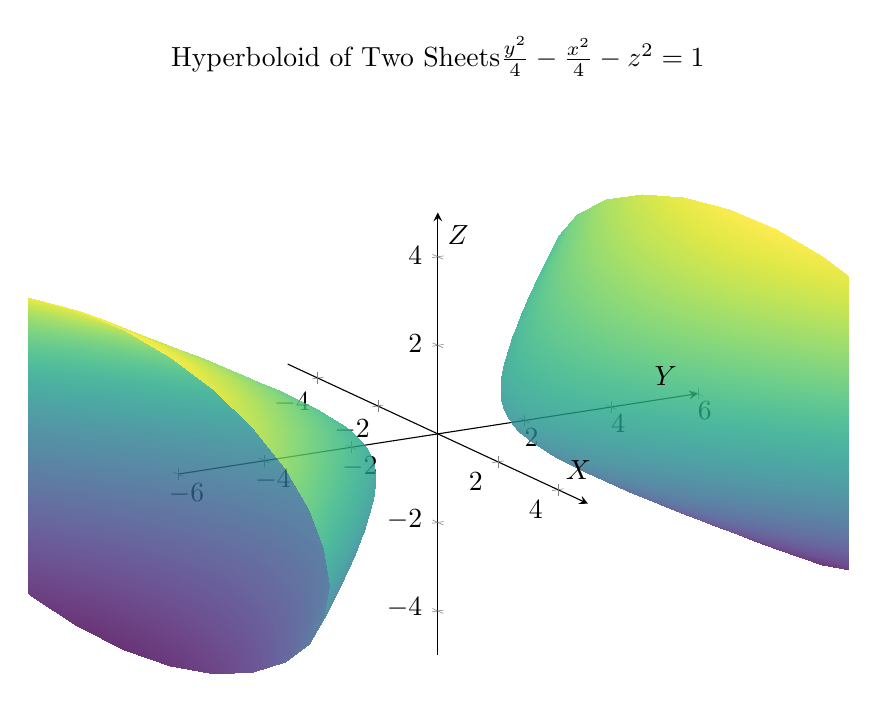
\begin{tikzpicture}
\begin{axis}[
    width=12cm,
    height=10cm,
    xlabel={$X$},
    ylabel={$Y$},
    zlabel={$Z$},
    title={Hyperboloid of Two Sheets \\ $\frac{y^2}{4} - \frac{x^2}{4} - z^2 = 1$},
    view={60}{20},
    grid=none,
    axis lines=center,
    enlargelimits=false,
    colormap/viridis,
    z buffer=sort,
    xmin=-5, xmax=5,
    ymin=-6, ymax=6,
    zmin=-5, zmax=5,
]

% Upper sheet
\addplot3[
    surf,
    domain=0:2,
    y domain=0:360,
    samples=30,
    samples y=30,
    opacity=0.8,
    shader=interp,
] ({2*sinh(x)*cos(y)}, {2*cosh(x)}, {sinh(x)*sin(y)});

% Lower sheet
\addplot3[
    surf,
    domain=0:2,
    y domain=0:360,
    samples=30,
    samples y=30,
    opacity=0.8,
    shader=interp,
] ({2*sinh(x)*cos(y)}, {-2*cosh(x)}, {sinh(x)*sin(y)});

\end{axis}
\end{tikzpicture}
\end{document}